\chapter{Phương pháp đề xuất}

Chương này trình bày chi tiết phương pháp bộ nhớ sự kiện có bằng chứng cho chính sách VLA điều khiển robot một tay. Phương pháp được thiết kế nhằm giải quyết bài toán quan sát một phần trong các tác vụ thao tác chuỗi dài có tính chất lặp lại, che khuất hoặc phụ thuộc thứ tự lịch sử. Trong quá trình robot thực thi đoạn hành động, một bộ điều phối giám sát trực tiếp các thay đổi bằng chứng trong bộ nhớ để kích hoạt quyền ngắt và tái truy vấn chính sách khi cần thiết. Các phân tích lý thuyết, thuật toán và mô hình thích ứng được trình bày tổng quát, trước khi cụ thể hóa trên bộ tiêu chuẩn LIBERO-Mem và hai mô hình nền SmolVLA, X-VLA. Vì bộ nhớ được đưa vào chính sách qua đầu vào ngôn ngữ, các thành phần ghi, chiếu và điều phối không phụ thuộc vào kiến trúc của mô hình nền.

\section{Phát biểu bài toán và tổng quan kiến trúc}

Như đã phân tích tại Mục~\ref{sec:pomdp}, trong các tác vụ thao tác có tính lặp lại hoặc che khuất, các quan sát cảm biến tức thời $o_t$ có thể hoàn toàn đồng dạng dù trạng thái tiến độ thực tế $z_t$ khác biệt. Việc cung cấp toàn bộ lịch sử tương tác thô $h_t = (o_0, a_0, \ldots, a_{t-1}, o_t)$ cho mô hình VLA dưới dạng chuỗi video hay nhiều khung hình quá khứ sẽ nhanh chóng làm bùng nổ số lượng token đầu vào, vượt quá ngân sách ngữ cảnh và làm suy giảm tần số điều khiển của các mô hình VLA nhỏ gọn. Do đó, mục tiêu cốt lõi của phương pháp đề xuất là xây dựng một cơ chế bộ nhớ trung gian có cấu trúc: liên tục trích xuất và tích lũy các sự kiện quan hệ thực thể vào bộ nhớ sự kiện $M_t$, sau đó chiếu các dữ kiện có căn cứ thành chuỗi văn bản ngắn gọn $C_q$ dưới ngân sách token hữu hạn $B$ tại thời điểm truy vấn $q$.

Hình~\ref{fig:architecture} tóm tắt vòng điều khiển qua bốn khối: bộ nhớ sự kiện, chính sách VLA, bộ điều phối và mô phỏng robot. Bộ nhớ sự kiện gồm bộ ghi trạng thái và bộ chiếu ngôn ngữ. Đường nét đứt màu xám biểu thị luồng dữ kiện cập nhật từ bộ nhớ đến bộ điều phối. Mũi tên đỏ biểu thị yêu cầu truy vấn sớm khi có dữ kiện mới đủ căn cứ.

\begin{equation}
\begin{aligned}
M_t &= U(M_{t-1}, o_t, a_{t-1}),\\
C_q &= R_B(\ell, M_q),\qquad |\operatorname{Enc}(C_q)| \le B,\\
A_q &\sim \pi_{\theta,\phi}(\cdot \mid o_q, C_q).
\end{aligned}
\label{eq:core-transforms}
\end{equation}

\begin{figure}[htbp]
\centering
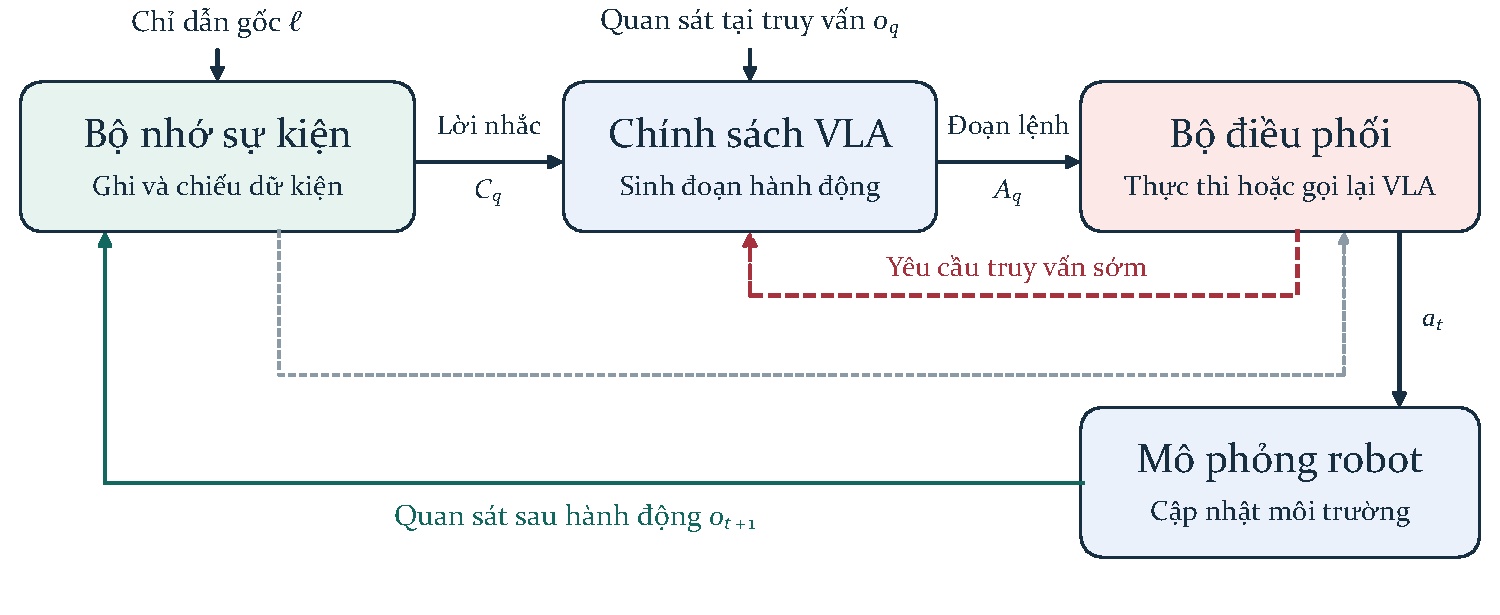
\includegraphics[width=\linewidth]{figures/vong-dieu-khien.pdf}
\caption{Vòng điều khiển VLA có bộ nhớ sự kiện}
\label{fig:architecture}
\end{figure}

%  Bộ đọc trích xuất dữ kiện có căn cứ để chiếu thành văn bản cho VLA sinh đoạn hành động. Bộ điều phối giám sát trực tiếp thay đổi trong bộ nhớ để kích hoạt quyền ngắt đoạn hành động
Trong đó $\ell$ là câu lệnh chỉ dẫn ngôn ngữ tổng thể của tác vụ, $M_t$ là trạng thái bộ nhớ sự kiện tại bước $t$, $C_q$ là ngữ cảnh ngôn ngữ được bộ đọc $R_B$ trích xuất và biểu diễn dưới ngân sách $B$ token tại thời điểm truy vấn $q$, và $A_q = (a_q, a_{q+1}, \ldots, a_{q+H-1})$ là đoạn hành động gồm $H$ bước liên tiếp do chính sách $\pi_{\theta,\phi}$ sinh ra từ quan sát hiện tại $o_q$ và ngữ cảnh $C_q$. Quy trình vận hành được điều phối khép kín: trước hết, bộ ghi cập nhật trạng thái bộ nhớ $M_t$ sau từng bước quan sát cảm biến $o_t$ và hành động vừa thực hiện $a_{t-1}$; thứ hai, tại mỗi bước truy vấn $q$, bộ đọc trích xuất các bằng chứng có căn cứ lịch sử, định dạng thành chuỗi văn bản ngắn $C_q$ không vượt quá $B$ token; thứ ba, chính sách VLA tiếp nhận cặp đầu vào $(o_q, C_q)$ để sinh đoạn hành động $A_q$; cuối cùng, bộ điều phối giám sát liên tục diễn biến của $M_t$ trong suốt quá trình robot thực thi đoạn hành động để quyết định có ngắt đoạn sớm hay không.

Tính an toàn của cơ chế này có thể được phân tích chặt chẽ qua lý thuyết xác suất sai số quyết định. Xét tình huống robot cần phân biệt hai trạng thái tiềm ẩn đồng xác suất (chẳng hạn vật nằm ở hộp X hoặc hộp Y) khi quan sát hiện tại hoàn toàn đồng nhất, sai số quyết định của chính sách phản xạ ngẫu nhiên là $1/2$. Giả sử bộ nhớ cung cấp câu trả lời với tỷ lệ bao phủ $c \in [0, 1]$ và tỷ lệ khẳng định sai là $\epsilon \in [0, 1]$. Áp dụng công thức xác suất toàn phần, kỳ vọng sai số quyết định của hệ thống được xác định bởi:

\begin{equation}
\mathbb E[\text{err}] = c\epsilon + \frac{1-c}{2} = \frac{1}{2} - c\left(\frac{1}{2} - \epsilon\right).
\label{eq:error-analysis}
\end{equation}

Phương trình~\eqref{eq:error-analysis} chỉ ra một kết quả lý thuyết quan trọng: kỳ vọng sai số toàn phần chỉ giảm so với chính sách phản xạ khi và chỉ khi tỷ lệ khẳng định sai thỏa mãn điều kiện $\epsilon < 1/2$. Ngược lại, nếu bộ nhớ đưa ra thông tin bị ảo giác với $\epsilon > 1/2$, việc tăng độ bao phủ $c$ sẽ làm tăng sai số toàn phần của hệ thống. Trong mô hình đơn giản này, việc giữ trạng thái \textit{chưa xác định} khi thiếu căn cứ quan sát tốt hơn việc suy đoán khi tỷ lệ khẳng định sai vượt $1/2$; mô hình chưa được kiểm chứng trên dữ liệu thực. Để tránh rò rỉ thông tin, kiến trúc thiết lập ranh giới phân tách độc lập hoàn toàn giữa nguồn thông tin của chính sách và nguồn đánh giá benchmark: bộ ghi và bộ đọc chỉ tiếp nhận dòng quan sát cảm biến được phép ($o_t$) mà không có quyền truy cập trạng thái môi trường đặc quyền, trong khi nhãn chân lý chỉ được sử dụng ở tầng đánh giá độc lập ngoại tuyến.

\section{Phương pháp bộ nhớ có bằng chứng}

\subsection{Cấu trúc bản ghi và tổ chức trạng thái}

Nhằm khắc phục triệt để hiện tượng mất dấu lịch sử và ảo giác thông tin, đơn vị lưu trữ cơ sở của bộ nhớ được thiết kế dưới dạng bản ghi sự kiện có cấu trúc tường minh:

\begin{equation}
f = (k, v, \sigma, \tau, \nu, I, \mathcal P).
\label{eq:record-tuple}
\end{equation}

Ý nghĩa toán học và chức năng của từng trường trong bộ bảy giá trị được định nghĩa như sau: trường khóa vị từ $k$ xác định tên quan hệ và vai trò định danh của các thực thể tham gia; trường giá trị $v$ lưu giữ giá trị chân lý, nhãn danh tính hoặc biến đếm tích lũy; trường trạng thái nhận thức $\sigma$ nhận giá trị trong tập gồm \textit{candidate} (ứng viên), \textit{confirmed} (xác nhận), \textit{unknown} (chưa rõ), \textit{conflicted} (mâu thuẫn), hoặc \textit{aborted} (hủy bỏ); trường $\tau$ ghi nhận thời điểm biến cố vật lý được ước lượng bắt đầu diễn ra trong môi trường thực; trường $\nu$ lưu giữ thời điểm xác nhận nhận thức ($\nu \ge \tau$), tức bước thời gian đầu tiên mà hệ thống tích lũy đủ chuỗi quan sát cảm biến phù hợp để chính thức xác nhận biến cố; trường khoảng thời gian hiệu lực $I = [t_{\mathrm{start}}, t_{\mathrm{end}}]$ xác định biên thời gian có giá trị của bản ghi (với sự kiện lịch sử thì $t_{\mathrm{end}} = \infty$, còn quan hệ hiện hành thì $t_{\mathrm{end}}$ kết thúc ngay khi có bằng chứng phủ định); và trường $\mathcal P$ lưu giữ tập chỉ mục nguồn gốc và căn cứ kiểm chứng gồm định danh khung ảnh cảm biến và tọa độ không gian để phục vụ truy vết nguyên nhân.

Để làm sáng tỏ ý nghĩa của cấu trúc trên, xét một bản ghi cụ thể ghi nhận biến cố robot đã hoàn thành việc đưa đồ vật A vào hộp X:

\begin{equation}
f_{\mathrm{ex}} = \Big(\underbrace{\text{In}(\text{obj}_A, \text{box}_X)}_{k},\ \underbrace{\text{true}}_{v},\ \underbrace{\text{confirmed}}_{\sigma},\ \underbrace{10}_{\tau},\ \underbrace{12}_{\nu},\ \underbrace{[10, \infty)}_{I},\ \underbrace{\mathcal P_{10:12}}_{\mathcal P}\Big).
\label{eq:record-example}
\end{equation}

Trong bản ghi mẫu này, tại bước thời gian vật lý $\tau = 10$, đồ vật A bắt đầu được đặt ổn định vào hộp X và tay kẹp robot mở ra. Tuy nhiên, để loại trừ rung lắc cảm biến, hệ thống yêu cầu điều kiện được thỏa mãn liên tục qua $p = 3$ quan sát liên tiếp, tức các bước 10, 11 và 12. Đến bước $\nu = 12$, khi vị từ hình học và trạng thái nhả kẹp được thỏa mãn liên tục, trạng thái nhận thức $\sigma$ chính thức được chuyển từ \textit{candidate} sang \textit{confirmed}. Khoảng hiệu lực $I = [10, \infty)$ phản ánh tính chất của một sự kiện lịch sử đã hoàn tất trong quá khứ (chân lý của biến cố này được bảo toàn vĩnh viễn trong tương lai của lượt thực thi), và tập căn cứ $\mathcal P_{10:12} = \{(\text{rgb}_t, \mathbf b_t^{\mathrm{obj}}, \text{grip}_t)\}_{t=10}^{12}$ lưu giữ đầy đủ mã định danh khung ảnh, tọa độ hộp bao và độ mở tay kẹp từ bước 10 đến 12 để phục vụ việc kiểm chứng và truy vết nguyên nhân khi cần thiết.

Việc phân tách ranh giới giữa thời điểm vật lý $\tau$ và thời điểm xác nhận nhận thức $\nu$ là một đóng góp thiết kế quan trọng. Một sự kiện thao tác có thể bắt đầu diễn ra ở bước $\tau = 10$, nhưng cảm biến cần quan sát thêm hai bước tiếp theo để xác nhận sự ổn định vật lý, dẫn tới thời điểm đủ căn cứ là $\nu = 12$. Trong trường hợp này, thông tin sự kiện tuyệt đối không được phép xuất hiện trong ngữ cảnh suy luận tại bước 10 hay 11, ngăn chặn triệt để hiện tượng rò rỉ thông tin tương lai trong cả pha huấn luyện lẫn pha suy luận.

Toàn bộ tri thức tích lũy của robot đến bước thời gian $t$ được tổ chức thành trạng thái bộ nhớ bốn thành phần:

\begin{equation}
M_t = (\mathcal O_t, \mathcal R_t, \mathcal E_t, \mathcal P_t).
\label{eq:memory-state}
\end{equation}

Trong đó $\mathcal O_t$ là tập hợp các thực thể và giả thuyết định danh đang được hệ thống duy trì, $\mathcal R_t$ là tập hợp các quan hệ trạng thái đang còn hiệu lực tại bước $t$, $\mathcal E_t$ là tập hợp các sự kiện lịch sử đã được xác nhận hoàn tất trong quá khứ, và $\mathcal P_t$ là chỉ mục tham chiếu bằng chứng và nguồn gốc dữ liệu.

\begin{figure}[htbp]
\centering
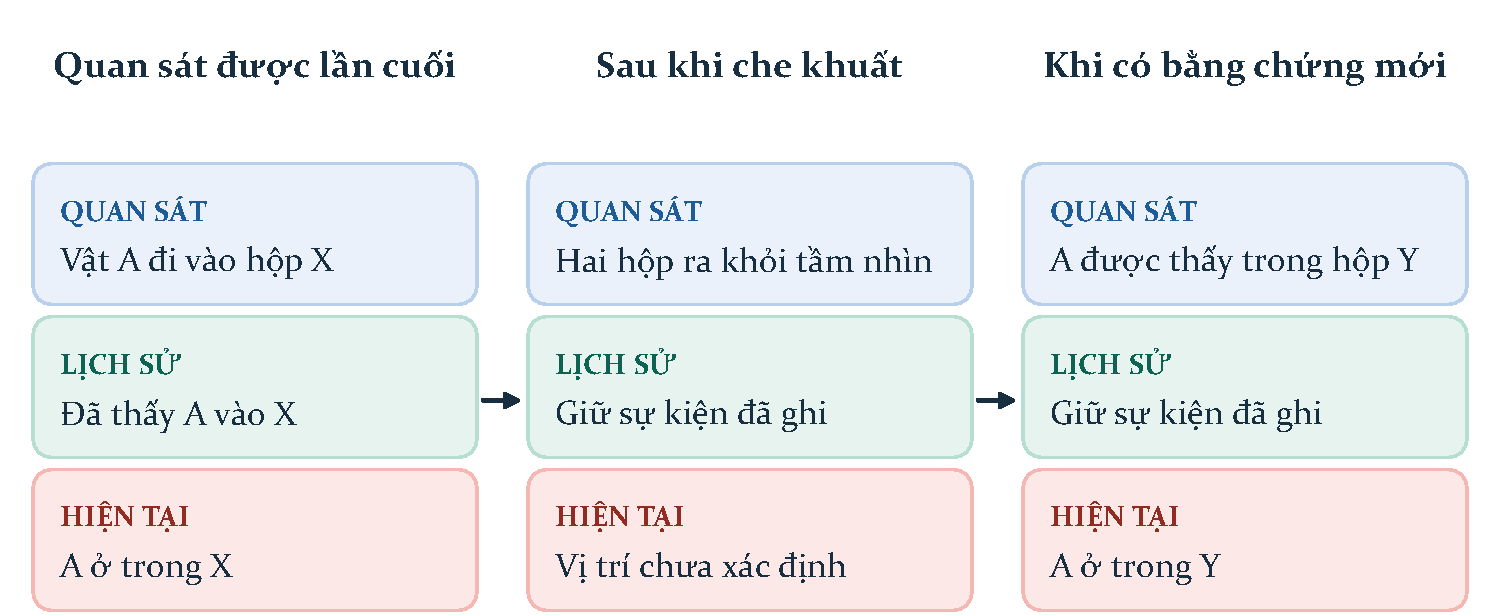
\includegraphics[width=.95\textwidth]{figures/su-kien-che-khuat.pdf}
\caption{Sự kiện lịch sử và quan hệ hiện tại khi vật bị che khuất}
\label{fig:memory-evidence-states}
\end{figure}

Như được minh họa ở Hình~\ref{fig:memory-evidence-states}, sự phân định giữa $\mathcal R_t$ và $\mathcal E_t$ phản ánh sự khác biệt căn bản về mặt nhận thức học. Sự kiện lịch sử ($\mathcal E_t$) mô tả một biến cố đã xảy ra trong quá khứ dựa trên quan sát thực tế tại thời điểm đó, có tính chân lý bất biến theo thời gian và không bị hủy bỏ bởi các diễn biến che khuất sau đó. Ngược lại, quan hệ hiện hành ($\mathcal R_t$) mô tả trạng thái không gian tại thời điểm hiện tại và chỉ có hiệu lực chừng nào các điều kiện bảo toàn vật lý được duy trì; nếu vật thể bị che khuất hoặc di chuyển khỏi tầm quan sát tin cậy, quan hệ trong $\mathcal R_t$ buộc phải chuyển trạng thái sang \textit{chưa xác định}. Cấu trúc này cho phép bộ nhớ đáp ứng linh hoạt cả ba dạng truy vấn trọng yếu: truy vấn không gian hiện tại từ $\mathcal R_t$, truy vấn ngữ cảnh quá khứ từ $\mathcal E_t$, và truy vấn tiến độ thao tác thông qua phép tổng hợp và đếm trên tập sự kiện $\mathcal E_t$.

\subsection{Nguyên lý trích xuất và kiểm định bằng chứng}

Để khung bộ nhớ có thể vận hành tổng quát trên nhiều tác vụ mà không bị phụ thuộc vào các ngưỡng tham số cục bộ, quá trình trích xuất và kiểm định bằng chứng được thiết kế dựa trên ba nguyên tắc cốt lõi: chuẩn hóa quan hệ hình học theo kích thước vật thể, bảo lưu danh tính thực thể khi bị che khuất, và khử nhiễu cảm biến thông qua cơ chế xác nhận trễ thời gian.

Trước hết, từ mỗi quan sát cảm biến $o_t$, hệ thống xác định vị trí và hộp bao của các thực thể liên quan. Nhằm loại bỏ hoàn toàn sự phụ thuộc vào góc đặt camera, cự ly quan sát và kích thước vật lý riêng của từng đồ vật, quan hệ không gian được đánh giá dựa trên độ dịch chuyển tương đối đã được chuẩn hóa theo kích thước của đối tượng mốc:

\begin{equation}
d_t = (\mathbf x_t^{\mathrm{obj}} - \mathbf x_t^{\mathrm{ref}}) - (\mathbf x_0^{\mathrm{obj}} - \mathbf x_0^{\mathrm{ref}}),\qquad
D_t = \left\| d_t \oslash \mathbf w_{\mathrm{ref}} \right\|_2.
\label{eq:scale-invariant-distance}
\end{equation}

Trong đó $\mathbf x_t^{\mathrm{obj}}$ và $\mathbf x_t^{\mathrm{ref}}$ lần lượt là tọa độ trung tâm của vật thể thao tác và đối tượng tham chiếu mốc tại bước $t$, $\mathbf w_{\mathrm{ref}}$ là kích thước hình học biểu kiến của đối tượng mốc, và $\oslash$ biểu thị phép chia theo từng thành phần tọa độ. Đại lượng vô hướng $D_t$ cung cấp một chỉ số đo khoảng cách tương đối không thứ nguyên, phản ánh mức độ thay đổi vị trí một cách nhất quán bất kể vật thể lớn hay nhỏ, đặt gần hay xa camera.

Thứ hai, nhằm duy trì tính nhất quán nhận thức trong suốt chuỗi thao tác, hệ thống cần bảo lưu chính xác danh tính của từng thực thể ngay cả khi xảy ra va chạm hay che khuất. Bằng cách liên kết các phát hiện thị giác tại bước $t$ với tập thực thể $\mathcal O_{t-1}$ dựa trên vị trí không gian kết hợp với đặc trưng diện mạo, hệ thống nhận biết liên tục đối tượng nào đang được thao tác. Khi một thực thể tạm thời bị che khuất bởi ngón kẹp robot hoặc di chuyển khỏi tầm nhìn của camera, trạng thái của nó được chuyển sang \textit{occluded} nhưng danh tính và lịch sử tương tác vẫn được duy trì trong bộ nhớ, thay vì bị xóa bỏ hoặc bị nhận diện nhầm thành một vật thể mới.

Thứ ba, do dữ liệu thị giác từ camera thường chịu ảnh hưởng bởi nhiễu hoặc sai số, hệ thống áp dụng cơ chế xác nhận trễ thời gian với độ dài cửa sổ $p$ quan sát. Một biến cố trạng thái không bao giờ được kích hoạt chỉ sau một quan sát riêng lẻ; thay vào đó, biến cố chỉ chính thức chuyển từ trạng thái ứng viên sang trạng thái xác nhận khi vị từ tương ứng duy trì giá trị thỏa mãn liên tục qua ít nhất $p$ bước quan sát kế tiếp nhau, trong đó $\phi_k$ là hàm vị từ ứng với khóa $k$:

\begin{equation}
\sigma_t = \text{confirmed} \iff \forall i \in [t - p + 1, t],\ \phi_k(o_i) = \text{true}.
\label{eq:temporal-hysteresis}
\end{equation}

Tiến trình thao tác tổng thể được quản lý bởi một máy trạng thái hữu hạn. Gọi $J_t$ là số chu kỳ thao tác đã bắt đầu, $\hat z_t$ là số chu kỳ đã hoàn thành hợp lệ được bộ nhớ xác nhận, $X_t$ là số chu kỳ bị hủy bỏ do vi phạm điều kiện an toàn, và $\chi_t$ là biến trạng thái chỉ thị chu kỳ hiện tại đang diễn ra ($\chi_t = 1$) hay hệ thống đang ở trạng thái nghỉ ($\chi_t = 0$). Tiến trình của hệ thống luôn thỏa mãn FSM invariant:

\begin{equation}
J_t - \hat z_t - X_t = \chi_t,\qquad \chi_t \in \{0, 1\}.
\label{eq:fsm-invariant}
\end{equation}

Bất biến~\eqref{eq:fsm-invariant} cho biết tại mọi bước, tổng số chu kỳ đã hoàn thành, đã hủy và đang diễn ra luôn bằng số chu kỳ đã bắt đầu, nên máy trạng thái không thể bỏ qua một chuyển tiếp. Bất biến này được kiểm tra bằng quy nạp theo từng chuyển tiếp của FSM: mỗi chuyển tiếp hợp lệ chỉ làm thay đổi đúng một trong các đại lượng $J_t$, $\hat z_t$, $X_t$ và giữ $\chi_t \in \{0,1\}$. Đặc tính nhân quả chặt chẽ của toàn bộ quy trình trích xuất và chiếu ngữ cảnh được khẳng định qua mệnh đề sau.

\textbf{Mệnh đề 1: Tính không nhìn trước của ngữ cảnh chiếu.} Giả sử hai quỹ đạo tương tác có cùng tiền tố quan sát và hành động đến bước truy vấn $q$, tức $h_q = h'_q$. Khi đó trạng thái bộ nhớ và ngữ cảnh chiếu tại bước $q$ là hoàn toàn đồng nhất:

\begin{equation}
h_q = h'_q \implies M_q = M'_q \implies R_B(\ell, M_q) = R_B(\ell, M'_q).
\label{eq:non-anticipatory}
\end{equation}

\textbf{Chứng minh.} Tại bước khởi đầu $t=0$, hai quỹ đạo có cùng cấu hình và quan sát ban đầu $o_0 = o'_0$, do đó $M_0 = M'_0$. Giả sử quy nạp rằng $M_{t-1} = M'_{t-1}$ với mọi $t \le q$. Vì hai tiền tố giống hệt nhau $h_q = h'_q$, ta có $o_t = o'_t$ và $a_{t-1} = a'_{t-1}$. Do quy tắc cập nhật $U$ là một hàm xác định, ta suy ra $M_t = U(M_{t-1}, o_t, a_{t-1}) = U(M'_{t-1}, o'_t, a'_{t-1}) = M'_t$. Áp dụng quy nạp đến bước $q$, ta thu được $M_q = M'_q$. Cuối cùng, vì phép chiếu $R_B$ chỉ đọc các bản ghi trong $M_q$ có $\nu \le q$, hai trạng thái bộ nhớ giống nhau sẽ sinh ra cùng một tập sự kiện được chọn $S_q = S'_q$ và cùng một chuỗi văn bản $C_q = C'_q$. $\blacksquare$

\begin{figure}[htbp]
\centering
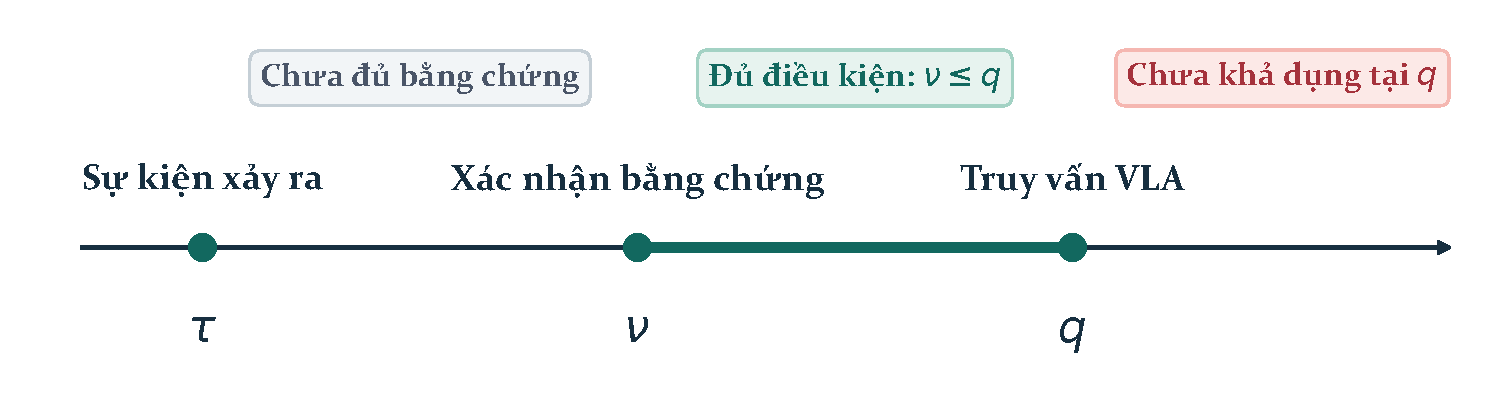
\includegraphics[width=.93\textwidth]{figures/truc-bang-chung.pdf}
\caption{Thời điểm xảy ra, xác nhận và truy vấn sự kiện}
\label{fig:memory_timeline}
\end{figure}

Mệnh đề 1 bảo đảm rằng ngữ cảnh được bộ nhớ cấp cho VLA hoàn toàn là hệ quả nhân quả của các quan sát quá khứ, loại bỏ khả năng mô hình học vẹt hoặc dựa trên rò rỉ tương lai như minh họa ở Hình~\ref{fig:memory_timeline}.

\subsection{Các trường hợp cụ thể với tác vụ}

Để áp dụng khung bộ nhớ trên các lớp tác vụ khác nhau, hệ thống định nghĩa một giao thức bộ nhớ theo tác vụ $T_{\mathrm{spec}} = (\Phi, \Delta, \mathcal{F})$, trong đó $\Phi$ là tập các hàm vị từ, $\Delta$ là tập các quy tắc chuyển trạng thái FSM, và $\mathcal{F}$ là định dạng chuỗi chiếu văn bản. LIBERO-Mem \cite{liberomem2025} chia mười tác vụ thành bốn nhóm năng lực bộ nhớ: OM (Object Motion, nhớ lịch sử chuyển động và trạng thái tương tác của từng vật thể), OS (Object Sequence, nhớ số lần và thứ tự tương tác), OR (Object Relations, nhớ quan hệ và vị trí giữa nhiều vật thể) và OO (Object Occlusion, nhớ danh tính và vị trí vật thể khi bị che khuất). Một tác vụ có thể thuộc nhiều nhóm. Bảng~\ref{tab:memory-task-families} tổng hợp nhóm năng lực và các primitive lịch sử cần thiết cho mười tác vụ này.

\begingroup\small\setlength{\tabcolsep}{4pt}\renewcommand{\arraystretch}{1.12}
\begin{longtable}{>{\raggedright\arraybackslash}p{.12\textwidth}|>{\raggedright\arraybackslash}p{.28\textwidth}|>{\raggedright\arraybackslash}p{.52\textwidth}}
\caption{Dạng thông tin lịch sử theo tác vụ LIBERO-Mem}\label{tab:memory-task-families}\\
\toprule
\textbf{Tác vụ} & \textbf{Lớp bài toán lịch sử} & \textbf{Primitive trừu tượng cần biểu diễn} \\
\midrule\endfirsthead
\toprule
\textbf{Tác vụ} & \textbf{Lớp bài toán lịch sử} & \textbf{Primitive trừu tượng cần biểu diễn} \\
\midrule\endhead
\bottomrule\endfoot
T1 & Đơn chu kỳ (OM) & Một chu kỳ nhấc và hoàn nguyên vật thể về mốc ban đầu \\
T2 & Tương tác trạng thái (OM) & Trạng thái tương tác tiếp xúc giữa hai vật thể \\
T3 & Đa chu kỳ ngắn (OM, OS) & Đếm và phân biệt tiến độ ba chu kỳ thao tác lặp lại \\
T4 & Đa chu kỳ tương tác (OM, OS) & Đếm số lần tương tác có chủ đích với vật thể \\
T5 & Đa chu kỳ trung bình (OM, OS) & Duy trì bộ đếm sự kiện qua năm chu kỳ liên tiếp \\
T6 & Đa chu kỳ dài (OM, OS) & Duy trì bộ đếm sự kiện qua bảy chu kỳ liên tiếp \\
T7 & Hoán đổi không gian (OM, OR) & Theo dõi quan hệ vị trí của hai vật thể qua ba mốc hoán đổi \\
T8 & Xoay vòng vị trí (OM, OR) & Theo dõi danh tính và vị trí của ba vật thể qua chuỗi xoay vòng \\
T9 & Vật chứa di chuyển (OM, OO) & Duy trì quan hệ chứa khi đối tượng chứa bị di chuyển \\
T10 & Phân biệt vật chứa (OM, OO) & Phân biệt vật chứa có chứa đồ vật với vật chứa rỗng sau che khuất \\
\end{longtable}
\endgroup

Khung giao thức này khẳng định tính tổng quát của phương pháp: các dạng bài toán từ đếm chu kỳ thao tác (OM/OS), theo dõi hoán đổi vị trí (OR) đến duy trì quan hệ vật chứa khi che khuất (OO) đều có thể được chuẩn hóa dưới dạng các bản ghi sự kiện có bằng chứng $f = (k, v, \sigma, \tau, \nu, I, \mathcal P)$.

Để chứng minh tính khả thi, nghiên cứu xây dựng một trường hợp cụ thể hóa điển hình: Bộ theo dõi chu kỳ thao tác lặp lại đối với vật thể trên mặt bàn bằng camera RGB. Trong trường hợp hiện thực này, vật thể thao tác và mốc tham chiếu được trích xuất tọa độ thông qua các hộp bao thị giác 2D từ camera ngoài và camera cổ tay. Gọi $\mathbf b_t$ và $\mathbf q_t$ lần lượt là tâm mép dưới của hộp bao vật thể và mốc vị trí tại bước $t$, $(w_b, h_b)$ là kích thước hộp bao vật thể tại thời điểm xác lập mốc ban đầu. Các đại lượng hình học tương đối được tính toán theo Phương trình~\eqref{eq:scale-invariant-distance}:

\begin{equation}
d_t = (\mathbf b_t - \mathbf q_t) - (\mathbf b_0 - \mathbf q_0),\qquad
D_t = \left\| d_t \oslash (w_b, h_b) \right\|_2,\qquad
L_t = -d_{t,y} / h_b.
\label{eq:case-study-geometry}
\end{equation}

Trong đó $D_t$ đo độ lệch mặt bằng đã chuẩn hóa, $L_t$ đo độ dịch chuyển nâng lên theo phương thẳng đứng của ảnh. Bảng~\ref{tab:case-study-thresholds} trình bày chi tiết các tiêu chí định lượng được cấu hình cho trường hợp cụ thể hóa này.

\begingroup\small\setlength{\tabcolsep}{4pt}\renewcommand{\arraystretch}{1.15}
\begin{longtable}{>{\raggedright\arraybackslash}p{\dimexpr 0.25\textwidth-2\tabcolsep\relax}|>{\raggedright\arraybackslash}p{\dimexpr 0.35\textwidth-2\tabcolsep\relax}|>{\raggedright\arraybackslash}p{\dimexpr 0.4\textwidth-2\tabcolsep\relax}}
\caption{Ngưỡng theo dõi chu kỳ thao tác}\label{tab:case-study-thresholds}\\
\toprule
\textbf{Đại lượng kiểm tra} & \textbf{Tiêu chí định lượng} & \textbf{Vai trò nhận thức trong quy trình} \\
\midrule\endfirsthead
\toprule
\textbf{Đại lượng kiểm tra} & \textbf{Tiêu chí định lượng} & \textbf{Vai trò nhận thức trong quy trình} \\
\midrule\endhead
\bottomrule\endfoot
Điểm tin cậy phát hiện & $s_{\mathrm{det}} \ge 0{,}15$ & Lọc các đề xuất hộp bao đạt ngưỡng chất lượng \\
Ứng viên rời mốc & $L_t \ge 0{,}40$ và ra khỏi vùng lân cận mốc & Xác định thời điểm vật thể bắt đầu được nâng lên \\
Ứng viên quay về mốc & $D_t \le 0{,}30$, tỷ lệ rộng $[0{,}6; 1{,}5]$, cao $[0{,}3; 1{,}5]$ & Nhận diện vật thể đã quay về vùng không gian của mốc \\
Trạng thái ổn định & Độ dịch tâm mép dưới chuẩn hóa $\le 0{,}15$ & Xác nhận vật thể đã ổn định vị trí, không còn chuyển động \\
Tay kẹp mở hoàn toàn & Tổng độ mở hai khớp ngón kẹp $\ge 0{,}055$ m & Căn cứ vật lý bổ trợ xác nhận robot đã nhả vật thể \\
Xác nhận trễ thời gian & Duy trì phù hợp qua $p = 3$ bước liên tiếp & Cửa sổ xác nhận chống nhiễu đơn khung hình \\
Liên kết mốc tham chiếu & Khoảng cách 2D với mốc $\le 0{,}20$ và IoU $\ge 0{,}10$ & Kiểm tra vật thể đã hoàn nguyên đúng tọa độ ban đầu \\
\end{longtable}
\endgroup

Quy tắc sinh sự kiện hoàn thành chu kỳ được cụ thể hóa bằng điều kiện logic kết hợp đa phương thức:

\begin{equation}
\operatorname{Event}_{\mathrm{cycle\_complete}}(t) \iff
\left(
\begin{aligned}
&\text{State}_{t-1} = \text{lifted} \;\land\; D_t \le 0{,}30 \;\land\; L_t \le 0{,}15 \\
&\land\; \operatorname{Stable}(t, p) \;\land\; \operatorname{GripperOpen}(t)
\end{aligned}
\right).
\label{eq:event-rule-instantiation}
\end{equation}

Khi điều kiện Phương trình~\eqref{eq:event-rule-instantiation} thỏa mãn, bộ ghi ghi nhận một sự kiện hoàn thành chu kỳ mới vào $\mathcal E_t$, cập nhật bộ đếm tiến độ $\hat z_t \leftarrow \hat z_{t-1} + 1$, chuyển trạng thái FSM về $\text{idle}$, và giải phóng biến theo vết để sẵn sàng cho chu kỳ tiếp theo nếu tác vụ yêu cầu.

\section{Quy trình huấn luyện thích ứng}
\label{sec:adaptation}

Để chính sách VLA có khả năng tiếp nhận và khai thác hiệu quả tín hiệu bộ nhớ mà không phá vỡ khả năng thao tác cơ sở đã học trong giai đoạn tiền huấn luyện, khóa luận xây dựng một quy trình huấn luyện thích ứng có kiểm soát. Quy trình gồm ba bước dùng chung cho mọi mô hình nền; chỉ tập tham số được cập nhật ở bước thứ ba phụ thuộc vào kiến trúc cụ thể.

Trước hết, từ tập dữ liệu quỹ đạo mẫu chuyên gia, hệ thống áp dụng cơ chế chạy lại bộ ghi ngoại tuyến để sinh các mẫu huấn luyện theo đúng tiền tố nhân quả. Tại mỗi điểm truy vấn mẫu $q$, bộ ghi chỉ xử lý chuỗi quan sát quá khứ $o_{0:q}$ để tạo ra trạng thái bộ nhớ $M_q$ và chuỗi văn bản tương ứng $C_q = R_B(\ell, M_q)$. Mẫu huấn luyện được cấu trúc thành bộ ba $(o_q, C_q, A_q^{\mathrm{demo}})$, trong đó $A_q^{\mathrm{demo}}$ là đoạn $H$ hành động liên tiếp của chuyên gia bắt đầu từ bước $q$. Việc tạo mẫu ngoại tuyến nghiêm ngặt này loại bỏ hoàn toàn nguy cơ rò rỉ thông tin tương lai vào ngữ cảnh huấn luyện.

Thứ hai, để giải quyết hiện tượng quên thảm khốc khi tinh chỉnh trên dữ liệu mới, nghiên cứu áp dụng chiến lược lấy mẫu cân bằng hai miền dữ liệu. Tập dữ liệu huấn luyện được hòa trộn đồng đều theo tỷ lệ $1:1$ giữa tập dữ liệu có bộ nhớ $\mathcal D_{\mathrm{mem}}$ (gồm các quỹ đạo thao tác đa chu kỳ kèm ngữ cảnh tiến độ) và tập dữ liệu thao tác cơ sở $\mathcal D_{\mathrm{base}}$ (các tác vụ đơn lẻ không kèm bộ nhớ). Mục tiêu tối ưu hóa được xác định bởi hàm mất mát Flow Matching kết hợp trên cả hai miền dữ liệu:

\begin{equation}
\min_\phi \frac{1}{2} \mathbb E_{(o, C, A) \sim \mathcal D_{\mathrm{base}}} \mathcal L_{\mathrm{flow}}(\theta, \phi; o, C, A) + \frac{1}{2} \mathbb E_{(o, C, A) \sim \mathcal D_{\mathrm{mem}}} \mathcal L_{\mathrm{flow}}(\theta, \phi; o, C, A).
\label{eq:training-loss}
\end{equation}

Trong đó $\theta$ biểu thị các trọng số được đóng băng của mô hình nền, $\phi$ là tập tham số thích ứng được tối ưu, và $\mathcal L_{\mathrm{flow}}$ là hàm mất mát hồi quy trường vận tốc dòng chảy dòng hành động.

Thứ ba, tập tham số thích ứng $\phi$ được chọn theo kiến trúc của từng mô hình nền, trong khi dữ liệu, ngân sách cập nhật và cách tạo lời nhắc giữ nguyên giữa F0 và F1. Với SmolVLA, nghiên cứu thích ứng action expert bằng LoRA như Hình~\ref{fig:smolvla-lora}: các phép chiếu truy vấn $W_q$ và giá trị $W_v$ trong các tầng attention của action expert được bổ sung nhánh hạng thấp $W + \frac{\alpha}{r} B_{\mathrm{L}} A_{\mathrm{L}}$, với hạng $r = 16$ và hệ số tỉ lệ $\alpha = 32$. Quá trình huấn luyện cập nhật 645.120 tham số LoRA và giữ cố định các trọng số gốc của action expert, bộ mã hóa ảnh SigLIP, mô hình ngôn ngữ SmolLM2 và các mô-đun còn lại. Với X-VLA, tập $\phi$ gồm các ma trận LoRA và một số mô-đun được huấn luyện đầy đủ, tổng cộng khoảng 11,87 triệu tham số; cấu hình chi tiết được nêu ở Mục~\ref{sec:xvla-setup}.

\begin{figure}[htbp]
\centering
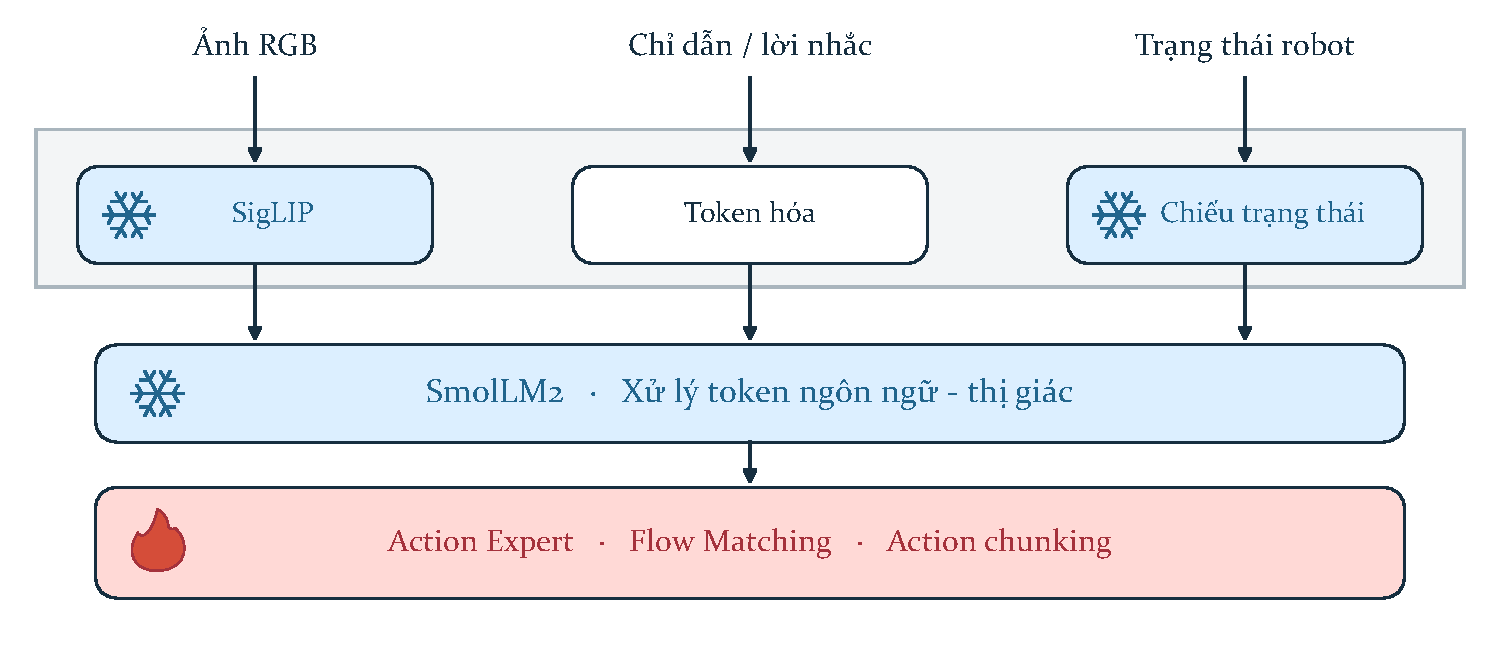
\includegraphics[width=.96\linewidth]{figures/smolvla-lora.pdf}
\caption{Phần đóng băng và phần tinh chỉnh LoRA trong SmolVLA}
\label{fig:smolvla-lora}
\end{figure}

\section{Suy luận và điều phối hành động theo thời gian thực}

Trong pha triển khai vận hành trực tuyến, chính sách VLA tích hợp bộ nhớ phải đáp ứng hai yêu cầu khắt khe: tuân thủ nghiêm ngặt ngân sách độ dài token đầu vào để duy trì tần số suy luận cao, và điều phối nhịp thực thi hành động linh hoạt nhằm phản ứng kịp thời với các biến cố môi trường.

Về mặt biểu diễn ngữ cảnh, bộ đọc áp dụng cơ chế chiếu nén có kiểm soát ngân sách: từ trạng thái bộ nhớ hiện tại $M_q$, bộ đọc lọc các bản ghi có căn cứ nhân quả $\nu \le q$, còn hiệu lực thời gian và có liên quan trực tiếp đến chỉ dẫn tác vụ $\ell$ để định dạng thành chuỗi văn bản tự nhiên $C_q$:

\begin{equation}
S_q = \operatorname{Select}(\ell, M_q, B),\qquad C_q = \operatorname{Render}(\ell, S_q),\qquad |\operatorname{Enc}(C_q)| \le B.
\label{eq:context-projection}
\end{equation}

Ngân sách độ dài được ấn định nghiêm ngặt ở mức $B = 48$ token cho toàn bộ văn bản đầu vào. Quy định này bảo đảm số lượng token đưa vào mô hình VLA luôn là một hằng số cố định, không phụ thuộc vào độ dài thời gian của quỹ đạo hay số lượng sự kiện đã tích lũy trong quá khứ, nên chi phí văn bản không tăng theo độ dài lượt chạy.

Về mặt điều phối thực thi, trong mô hình Action Chunking truyền thống, robot thực thi liên tục toàn bộ $H$ hành động trong đoạn theo chu kỳ cố định $s$ bước mới tái truy vấn VLA một lần. Nhược điểm lớn của cơ chế cố định này là độ trễ phản xạ cao: nếu một biến cố then chốt xảy ra ngay ở đầu đoạn hành động (chẳng hạn vật đã rơi vào đúng đích ở bước thứ 2 của đoạn $s = 10$), robot vẫn phải thực hiện 8 hành động còn lại trước khi nhận được trạng thái mới, gây lãng phí hoặc thao tác thừa. Để khắc phục, hệ thống triển khai cơ chế ngắt đoạn hành động động dựa trên bằng chứng: bộ điều phối giám sát liên tục diễn biến của $M_t$ sau mỗi bước thực thi hành động $t$. Khi phát hiện một thay đổi bằng chứng ngữ nghĩa có liên quan được duy trì ổn định qua $p$ quan sát liên tiếp và robot đã hoàn thành tối thiểu $k_{\min}$ hành động từ lần truy vấn trước, thời điểm truy vấn tiếp theo $q'$ được kích hoạt sớm. Gọi $e_t \in \{0,1\}$ là chỉ báo bằng chứng mới đã được xác nhận tại bước $t$, ta có:

\begin{equation}
q' = \min\!\left(q + s,\ \inf\{t > q : t - q \ge k_{\min},\ e_t = 1\}\right).
\label{eq:dynamic-preemption}
\end{equation}

Như minh họa tại Hình~\ref{fig:evidence-requery}, khi điều kiện ngắt được thỏa mãn tại $q'$, bộ điều phối lập tức hủy bỏ các hành động chưa thực thi trong đoạn cũ, lấy quan sát mới $o_{q'}$, chiếu ngữ cảnh cập nhật $C_{q'}$ và kích hoạt VLA sinh đoạn hành động mới.

\begin{figure}[htbp]
\centering
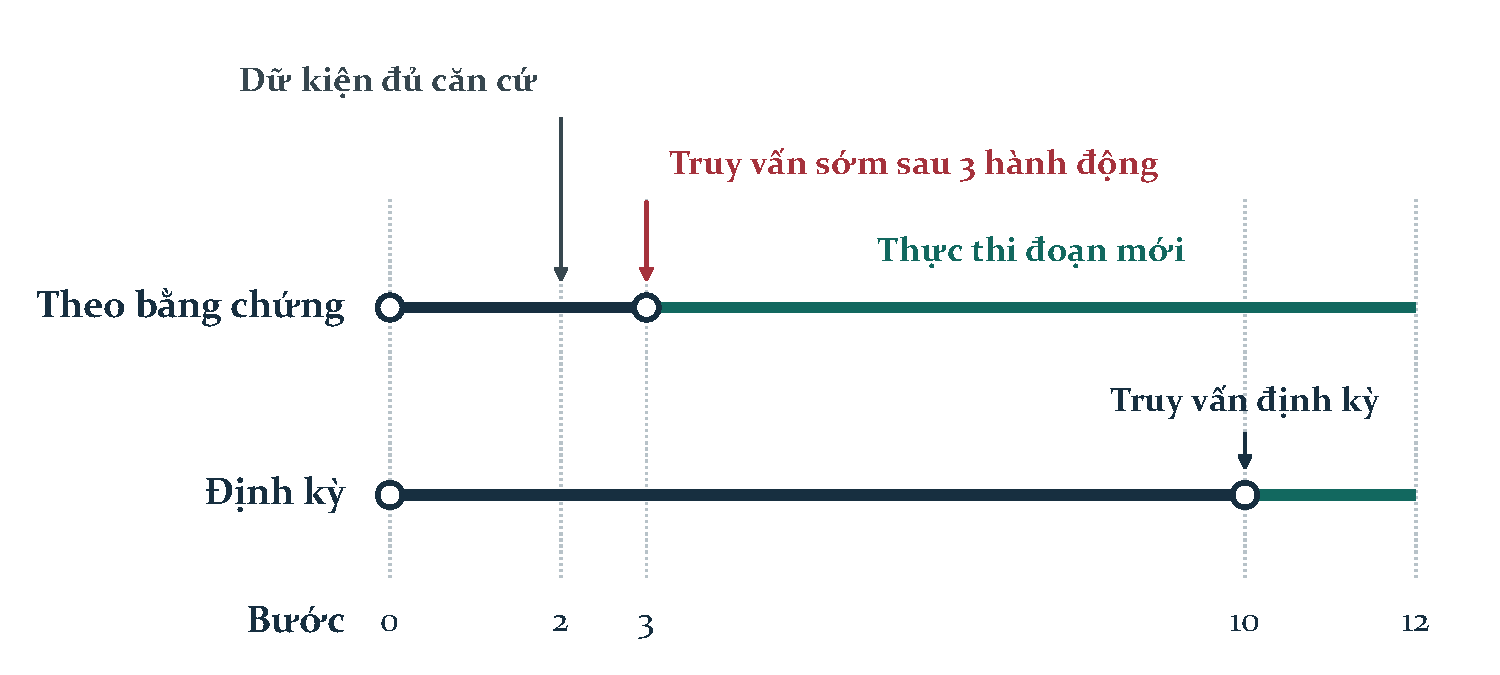
\includegraphics[width=.94\textwidth]{figures/truy-van-som.pdf}
\caption{Truy vấn sớm khi có bằng chứng mới}
\label{fig:evidence-requery}
\end{figure}

Hiệu quả phản ứng của cơ chế ngắt động có thể được chứng minh qua định lý chặn trên thời gian trễ.

\textbf{Mệnh đề 2: Chặn trên của độ trễ với biến cố mới.} Giả sử robot đang thực thi đoạn hành động được sinh tại bước $q$. Một biến cố trạng thái mới xuất hiện trong môi trường tại thời điểm $r$ (với $q < r \le q + s$) và duy trì liên tục. Nếu không có biến cố nào khác kích hoạt trước đó, thời điểm tái truy vấn chính sách $q'$ thỏa mãn:

\begin{equation}
q' = \min(q + s,\ \max(q + k_{\min},\ r + p - 1)).
\label{eq:latency-formula}
\end{equation}

Hệ quả là số bước hành động robot tiếp tục sử dụng đoạn điều khiển cũ sau khi biến cố xuất hiện, trong đó $r$ là thời điểm bộ ghi bắt đầu quan sát thấy biến cố, bằng:

\begin{equation}
q' - r = \min\!\big(q + s - r,\ \max(q + k_{\min} - r,\ p - 1)\big) \le q + s - r.
\label{eq:latency-bound}
\end{equation}

\textbf{Chứng minh.} Biến cố xuất hiện tại bước $r$. Do quy tắc lọc trễ thời gian đòi hỏi $p$ quan sát liên tiếp để xác nhận, thời điểm sớm nhất biến cố được xác nhận là $t_{\mathrm{confirm}} = r + p - 1$, tại đó $e_t = 1$. Đồng thời, cơ chế điều phối đòi hỏi robot phải thực thi tối thiểu $k_{\min}$ hành động từ lần truy vấn trước, tức $t \ge q + k_{\min}$. Do đó, bước thời gian sớm nhất thỏa mãn đồng thời cả hai điều kiện là $t = \max(q + k_{\min}, r + p - 1)$. Mặt khác, lịch truy vấn định kỳ chặn trên thời điểm gọi tiếp theo tại $q + s$. Kết hợp hai điều kiện, ta thu được $q' = \min(q + s, \max(q + k_{\min}, r + p - 1))$. Trừ $r$ ở hai vế của công thức trên ta được độ trễ nêu ở phương trình sau. Độ trễ thực tế của bộ ghi, được đo ở Chương 4 là từ 4 đến 30 bước đối với bộ ghi thị giác, cộng thêm vào $r$. $\blacksquare$

Công thức Phương trình~\eqref{eq:latency-formula} cho thấy rõ sự linh hoạt của cơ chế: khi biến cố được xác nhận sớm ($r + p - 1 < q + s$), hệ thống truy vấn lại ngay khi đã thực thi tối thiểu $k_{\min}$ hành động, nên độ trễ phản ứng nhỏ hơn so với việc thực thi hết chu kỳ $s$.

Bộ điều phối có thể mở rộng sang suy luận bất đồng bộ, trong đó luồng điều khiển và luồng truy vấn chạy song song và mỗi đề xuất được kiểm tra lại với phiên bản bộ nhớ khi hoàn tất. Tuy nhiên, hướng này không phải mục tiêu chính để cài đặt và đánh giá trong khóa luận này.

\textbf{Cơ chế dừng thực thi dựa trên bằng chứng bộ nhớ.}
\label{sec:method-memory-halt}

Bộ điều phối ở phần trước chỉ giải quyết bài toán thời điểm kích hoạt truy vấn lại chính sách, và mặc định giả định rằng mô hình VLA có thể tự nhận biết thời điểm kết thúc nhiệm vụ. Tuy nhiên, giả định này thường không thỏa mãn trong thực tế đối với các chính sách học từ quỹ đạo minh họa mẫu. Do dữ liệu minh họa thường kết thúc ngay khi mốc tác vụ cuối cùng đạt điều kiện, chính sách hiếm khi được quan sát trạng thái đứng yên sau khi hoàn thành, dẫn đến khuynh hướng tiếp tục thực thi thao tác thừa gây mất kết quả đã đạt, gọi là hiện tượng overshoot. Thông tin mà chính sách còn thiếu chính là tiến độ tích lũy theo thời gian, đúng với đại lượng mà bộ nhớ sự kiện liên tục cập nhật. Do đó, không gian quyết định của bộ điều phối được mở rộng thành ba trạng thái gồm tiếp tục thực thi, truy vấn lại sớm hoặc dừng hẳn thao tác, mà không làm xáo trộn không gian trọng số hay ngữ cảnh chiếu $C_q$.

Về mặt hình thức, gọi $z_t$ là tiến độ thực tế, $K$ là số chu kỳ mục tiêu của tác vụ, $T_c = \inf\{t: z_t \ge K\}$ là thời điểm hoàn thành và $T_o$ là thời điểm xảy ra thao tác thừa không thể phục hồi, quy ước $T_o = \infty$ khi chính sách tự bảo toàn kết quả. Khoảng thời gian $W = [T_c, T_o)$ xác định cửa sổ dừng hợp lệ. Trên tập các ranh giới truy vấn $\mathcal Q$, quy tắc dừng can thiệp được xác lập:
\begin{equation}
\tau = \min\{q \in \mathcal Q:\ \hat z_q \ge K\ \land\ g_q \ge \theta_g\ \land\ \psi_q\},\qquad a_t = a^{\mathrm{hold}}(x_\tau)\quad \forall t \ge \tau,
\label{eq:halt-rule}
\end{equation}
trong đó $\hat z_q$ là bộ đếm tiến độ do bộ nhớ cung cấp theo Phương trình~\eqref{eq:fsm-invariant}, $g_q \ge \theta_g$ là tín hiệu cảm nhận bản thể xác nhận tay kẹp đã nhả vật với ngưỡng độ mở $\theta_g = 0{,}055$~m, và $\psi_q$ là điều kiện xác thực bổ sung từ bộ nhớ mang giá trị đúng theo mặc định. Khi điều kiện thỏa mãn, trạng thái dừng được chốt vĩnh viễn: hệ thống ngắt toàn bộ các truy vấn tiếp theo tới chính sách VLA và duy trì tư thế đầu gắp hiện tại ở trạng thái kẹp mở. Vì mọi thành phần trong Phương trình~\eqref{eq:halt-rule} đều phụ thuộc thuần túy vào tiền tố lịch sử $h_q$, Mệnh đề~1 bảo đảm $\tau$ là một thời điểm dừng hợp lệ theo dòng thông tin quan sát, không sử dụng bất kỳ trạng thái ẩn hay cờ giám sát môi trường nào.

Nhằm tăng độ bao phủ khi một kênh cảm giác đơn lẻ bị gián đoạn, bộ đếm $\hat z_t$ hợp nhất thông tin từ nhiều nguồn theo từng pha kẹp vật thể, trong đó mỗi chu kỳ đóng mở tay kẹp chỉ được tích lũy tối đa một đơn vị tiến độ để triệt tiêu hoàn toàn nguy cơ đếm trùng lặp. Cấu hình cụ thể kết hợp hai luồng bằng chứng độc lập: bộ ghi nhận quan hệ thực thể thị giác theo Phương trình~\eqref{eq:event-rule-instantiation} và tín hiệu động học tiếp xúc từ cảm nhận bản thể, ghi nhận khi đầu gắp nâng lên tối thiểu $0{,}08$~m rồi hạ xuống trong phạm vi $0{,}03$~m theo phương thẳng đứng và $0{,}06$~m theo mặt phẳng ngang so với tọa độ ban đầu. Các tín hiệu động học này chỉ phục vụ riêng cho quyết định dừng ngoại vi, không đưa vào chuỗi ký tự $C_q$, giúp bảo toàn nguyên vẹn ngân sách token $B$ và phân phối ngôn ngữ đầu vào của mô hình nền.

Để đánh giá định lượng hiệu quả của cơ chế dừng, xét mô hình xác suất trên không gian quỹ đạo với các giả định tự nhiên: thời điểm dừng $\tau$ phụ thuộc nhân quả vào lịch sử quan sát; việc can thiệp dừng trong cửa sổ $W$ giữ được trạng thái thành công với xác suất $\rho$; việc dừng trước mốc $T_c$ được tính là thất bại do không tạo thêm tiến độ; và trạng thái thao tác thừa là trạng thái hấp thụ không thể đảo ngược. Đặt $p_c = \Pr(T_c \le T)$ là xác suất hoàn thành chu kỳ, $p_o = \Pr(T_o \le T \mid T_c \le T)$ là xác suất xảy ra lỗi lặp thao tác thừa, $r = \Pr(\tau \in W \mid \text{hoàn thành rồi lặp thừa})$ là xác suất can thiệp dừng thành công trong cửa sổ hợp lệ, cùng $f$ và $r'$ lần lượt là xác suất dừng non trước mốc $T_c$ và xác suất dừng trong cửa sổ $W$ đối với những lượt chạy vốn dĩ chính sách có thể tự bảo toàn thành công.

\textbf{Mệnh đề 3: Phân rã lợi ích và độ tin cậy của cơ chế dừng.} Dưới các giả định về tính nhân quả của thời điểm can thiệp, mức tăng xác suất thành công tổng thể $\Delta$ của chính sách khi tích hợp cơ chế dừng thỏa mãn:
\begin{equation}
\Delta = p_c \Big[ \underbrace{p_o\,\rho\,r}_{\text{lượng cứu được}} - \underbrace{(1 - p_o)\big(f + (1 - \rho)r'\big)}_{\text{lượng làm hỏng}} \Big].
\label{eq:halt-gain}
\end{equation}
Đồng thời, gọi $c$ là độ phủ nhận diện chu kỳ trong phạm vi độ trễ $D$, $\varepsilon$ là số tín dụng sai kỳ vọng trên mỗi pha kẹp, $\bar m$ là số pha kẹp kỳ vọng trước thời điểm $T_c$, và $\kappa_s$ là xác suất tồn tại thời điểm kiểm tra hợp lệ trong khoảng $[T_c + D, T_o)$. Khi đó, xác suất dừng non trước mốc hoàn thành bị chặn trên bởi $f \le \bar m \varepsilon$, và xác suất dừng thành công trong cửa sổ hợp lệ thỏa mãn chặn dưới $r \ge c^K (1 - \bar m \varepsilon) \kappa_s$.

\textbf{Chứng minh.} Lượt chạy không đạt đủ mốc $K$ sẽ thất bại bất kể có can thiệp dừng hay không. Những lượt chạy đạt mốc hoàn thành nhưng sau đó mắc lỗi lặp thao tác thừa vốn có kết quả gốc thất bại, và sẽ được khôi phục thành công khi và chỉ khi can thiệp dừng kịp thời trong cửa sổ $W$, đạt xác suất $\rho r$. Ngược lại, những lượt chạy vốn tự thành công sẽ bị làm hỏng nếu cơ chế kích hoạt dừng non trước $T_c$ với xác suất $f$, hoặc khi việc dừng giữ nguyên vị trí làm thất thoát điều kiện đích với xác suất $(1 - \rho)r'$. Phép cộng trên ba phân lớp quỹ đạo rời nhau cho ta công thức Phương trình~\eqref{eq:halt-gain}. Về giới hạn độ tin cậy, do trước thời điểm $T_c$ số chu kỳ thực tế nhỏ hơn $K$, điều kiện $\hat z_q \ge K$ chỉ có thể xuất hiện khi có ít nhất một tín dụng ghi nhận sai; theo bất đẳng thức Markov, xác suất này không vượt quá $\bar m \varepsilon$. Kết hợp với xác suất ghi nhận đủ $K$ chu kỳ trong độ trễ $D$ và tồn tại thời điểm kiểm tra hợp lệ, ta thu được chặn dưới cho tỷ lệ can thiệp thành công $r$. $\blacksquare$

Từ công thức Phương trình~\eqref{eq:halt-gain}, khi $\rho = 1$, điều kiện để cơ chế dừng mang lại lợi ích thực chất $\Delta > 0$ là tỷ số độ phủ trên độ sai lệch $r / f$ phải vượt qua ngưỡng $(1 - p_o) / p_o$. Đối với những chính sách hầu như không có năng lực tự dừng khi $p_o \to 1$, hệ thống luôn đạt lợi ích dương với mọi quy tắc dừng có độ phủ $r > 0$. Đáng chú ý, tỷ lệ dừng đúng $r$ suy giảm theo hàm mũ của số chu kỳ $K$ trong khi rủi ro dừng non $f$ chỉ tăng tuyến tính theo $\varepsilon$, khẳng định vai trò quyết định của việc hợp nhất đa nguồn tín hiệu nhằm nâng cao độ phủ chu kỳ mà không làm bùng nổ tín dụng sai lệch.

\textbf{Mệnh đề 4: Giá trị lý thuyết của bằng chứng bộ nhớ.} Xét phiếm hàm giá trị $V(\mathcal H) = \sup_\tau \Pr(\tau \in W)$ đại diện cho xác suất dừng tối ưu trong cửa sổ hợp lệ dưới dòng thông tin $\mathcal H$. Khi đó, thứ tự thông tin được xác lập:
\begin{equation}
V(\text{thời gian cố định}) \le V(\text{bằng chứng bộ nhớ}) \le V(\text{nguồn hoàn hảo}),
\label{eq:value-of-evidence}
\end{equation}
và mọi quy tắc dừng mù $\tilde\tau$ độc lập với trạng thái tương tác của lượt chạy đều thỏa mãn chặn trên $\Pr(\tilde\tau \in W) \le \max_t \Pr(T_c \le t < T_o) \le L_{\max} \max_u \Pr(T_c = u)$, trong đó $L_{\max}$ là độ dài lớn nhất của cửa sổ dừng hợp lệ.

\textbf{Chứng minh.} Do tập các thời điểm dừng xác định theo dòng thông tin thời gian thô là tập con của dòng thông tin bộ nhớ sự kiện, giá trị cận trên của bộ nhớ luôn không nhỏ hơn quy tắc chỉ dựa vào thời gian. Đối với một quy tắc dừng mù không phụ thuộc trạng thái, xác suất rơi vào cửa sổ dừng là trung bình của $\Pr(T_c \le t < T_o)$ theo phân phối thời gian, và biến cố này bị bao hàm trong tập các bước hoàn thành thỏa mãn $t - L_{\max} < T_c \le t$. Lấy cận trên theo bước thời gian hoàn thành $u$ cho ta kết quả cần chứng minh. $\blacksquare$

Mệnh đề~4 làm sáng tỏ nền tảng lý thuyết vì sao bằng chứng bộ nhớ vượt trội hơn các quy tắc định thời gian: khi thời điểm hoàn thành $T_c$ phân tán rộng trên các quỹ đạo khác nhau trong khi cửa sổ hợp lệ $L_{\max}$ lại tương đối ngắn, không tồn tại bất kỳ mốc thời gian cố định nào có thể dừng thành công cho mọi trường hợp. Bằng chứng bộ nhớ cung cấp tín hiệu neo động theo tiến trình vật lý thực tế, bảo đảm việc dừng thao tác diễn ra chính xác theo diễn biến từng quỹ đạo tương tác.
